\documentclass{standalone}
\usepackage{tikz} 
\usetikzlibrary{arrows, decorations.markings,decorations.text}
\usepackage{xcolor}
%\usepackage{BeamerColor}
\usepackage{microtype}
\usepackage{fourier}

\begin{document}

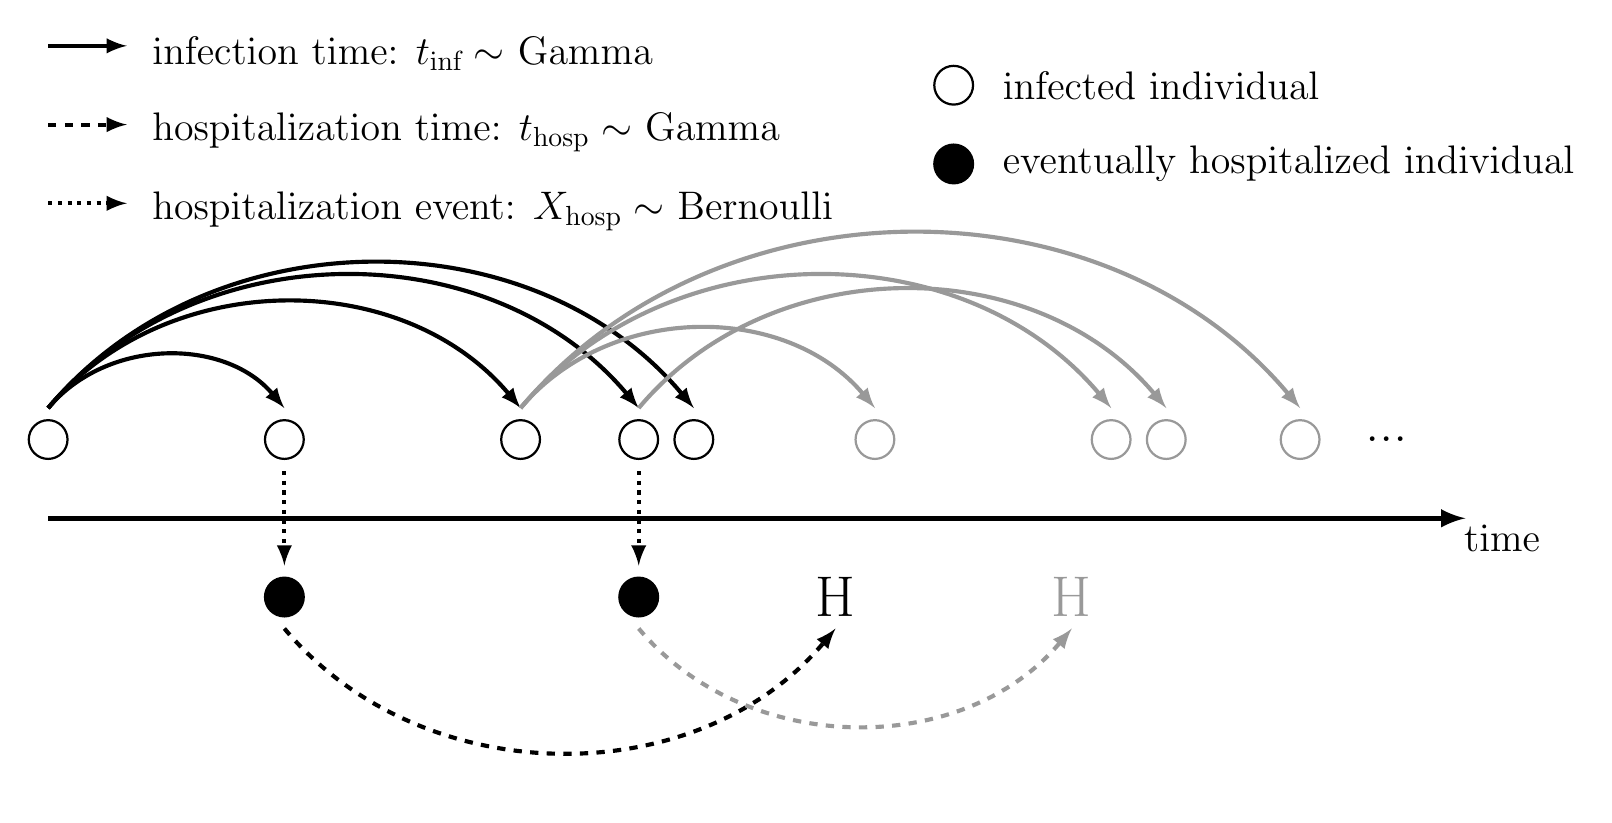
\begin{tikzpicture}
	
	% timeline
	\draw[-latex,line width=2pt,black] (0,0) -- (18,0) node [midway,above,sloped] {};
	\draw (18,-0.25) node[right=-4pt] {\Large time};

   	% 1st generation	
	\draw[fill=white,thick] (0,1) circle (7pt);
	
	% 2nd generation
	\draw[fill=white,thick] (3,1) circle (7pt);
	\draw[-latex,line width=1.5pt] (0,1.4) to[bend left=50] (3,1.4);
	
	\draw[fill=white,thick] (6,1) circle (7pt);
	\draw[-latex,line width=1.5pt] (0,1.4) to[bend left=50] (6,1.4);
	
	\draw[fill=white,thick] (7.5,1) circle (7pt);
	\draw[-latex,line width=1.5pt] (0,1.4) to[bend left=50] (7.5,1.4);
	
	\draw[fill=white,thick] (8.2,1) circle (7pt);
	\draw[-latex,line width=1.5pt] (0,1.4) to[bend left=50] (8.2,1.4);
	
	% 3rd generation
	\draw[color=black!40,fill=white,thick] (10.5,1) circle (7pt);
	\draw[-latex,color=black!40,line width=1.5pt] (6,1.4) to[bend left=50] (10.5,1.4);
	
	\draw[color=black!40,fill=white,thick] (13.5,1) circle (7pt);
	\draw[-latex,color=black!40,line width=1.5pt] (6,1.4) to[bend left=50] (13.5,1.4);
	
	\draw[color=black!40,fill=white,thick] (15.9,1) circle (7pt);
	\draw[-latex,color=black!40,line width=1.5pt] (6,1.4) to[bend left=50] (15.9,1.4);
	
	\draw[color=black!40,fill=white,thick] (14.2,1) circle (7pt);
	\draw[-latex,color=black!40,line width=1.5pt] (7.5,1.4) to[bend left=50] (14.2,1.4);
	
	% finish
	\draw (17,1) node {\huge ...};
	
	% Hospitalization events
	\draw[fill=black,thick] (3,-1) circle (7pt);
	\draw[-latex,line width=1.5pt,dotted] (3,0.6) to (3,-0.6);
	
	\draw[fill=black,thick] (7.5,-1) circle (7pt);
	\draw[-latex,line width=1.5pt,dotted] (7.5,0.6) to (7.5,-0.6);
	
	% Hospitalization arrows
	\draw (10,-1) node {\huge H};
	\draw[-latex,line width=1.5pt,dashed] (3,-1.4) to[bend right = 50] (10,-1.4);
	
	\draw (13,-1) node {\color{black!40}\huge H};
	\draw[-latex,color=black!40,line width=1.5pt,dashed] (7.5,-1.4) to[bend right = 50] (13,-1.4);
	
	% Legend
	\draw[-latex,line width=1.5pt,black] (0,6) -- (1,6);
	\draw (1.2,5.9) node[right=0pt] {\Large infection time: $t_{\textrm{\normalsize inf}} \sim$ Gamma}; 
	
	\draw[-latex,line width=1.5pt,black,dashed] (0,5) -- (1,5);
	\draw (1.2,4.9) node[right=0pt] {\Large hospitalization time: $t_{\textrm{\normalsize hosp}} \sim$ Gamma}; 
	
	\draw[-latex,line width=1.5pt,black,dotted] (0,4) -- (1,4);
	\draw (1.2,3.9) node[right=0pt] {\Large hospitalization event: $X_{\textrm{\normalsize hosp}} \sim$ Bernoulli}; 
	
	\draw[fill=white,thick] (11.5,5.5) circle (7pt);
	\draw (12,5.5) node[right=0pt] {\Large infected individual}; 
	
	\draw[fill=black,thick] (11.5,4.5) circle (7pt);
	\draw (12,4.5) node[right=0pt] {\Large eventually hospitalized individual}; 
	
\end{tikzpicture}						

\end{document}